\chapter{Framework para Proyectos Android de Ciencia Ciudadana}

\section{Frameworks}

	Un framework es un diseño abstracto para un tipo particular de aplicación,y generalmente consiste de un conjunto de clases. Estas clases pueden pertenecer a una librería o pueden ser específicas de la aplicación. Los frameworks se pueden construir sobre otros frameworks compartiendo clases abstractas.
	
	Brindan una manera de reutilizar código que es resistente frente a los intentos más comunes de reutilización. Los componentes independientes de una aplicación pueden ser reutilizados fácilmente, pero poder reutilizar la estructura que mantiene a los componentes juntos generalmente es posible copiando y editando. A diferencia de los programas esqueletos, que es el enfoque más convencional para reutilizar este tipo de código, los frameworks facilitan la tarea de asegurar que bajo requerimientos cambiantes la consistencia de todos sus componentes se va a mantener.
	
	Como hacen posible la reutilización en la granularidad más alta, diseñar un buen framework es mucho más difícil que diseñar una buena clase abstracta. También, tienden a ser específicos de la aplicación, a integrarse a otros frameworks mediante compartir clases abstractas, y a tener algunas clases abstractas especializadas para el framework. Diseñar un framework requiere experiencia y experimentación al igual que lo requiere el diseño de las clases abstractas de sus componentes.

\subsection{Frameworks de Caja Blanca y de Caja Negra}
\subsubsection{Frameworks de Caja Blanca}

	Una de las características importantes de un framework es que los métodos definidos por el usuario para extender el comportamiento van a ser invocados desde el interior del framework más que del código de la aplicación del usuario. A menudo hace las veces de programa principal coordinando y secuenciando las actividades de la aplicación. Esa inversión de control le permite al framework servir como esqueleto extensible. El código brindado por los usuarios en los métodos extienden el algoritmo genérico del framework para una aplicación en particular. 
	
	El comportamiento específico de una aplicación que utiliza un framework usualmente se define agregando métodos a las subclases o a una o más de sus clases. Cada método que se agrega a una subclase debe continuar con las convenciones internas que adoptan las superclases. Este tipo de framework se denomina de caja blanca (white-box) porque debe comprenderse cómo está implementado para poder utilizarlo.
	
	El principal problema de los frameworks de caja blanca es que cada aplicación requiere la creación de una numerosa cantidad  de subclases. Y aunque muchas de estas subclases creadas son simples, es su número lo que para un desarrollador con poca experiencia puede volver difícil comprender el diseño de una aplicación los suficiente como para modificarla.
	
	Un segundo problema es que un framework de caja blanca puede ser difícil de aprender a utilizar, ya que entender cómo se utliza es lo mismo que entender cómo está construido.
	
\subsubsection{Frameworks de Caja Negra}

	Otra manera de especializar un framework es incluir en él un conjunto de componentes que sean los que proveen el comportamiento específico de la aplicación. Cada uno de estos componentes debe entender un protocolo en particular. Todos o la mayoría de los componentes pueden tomarse de una librería de componentes. La interfaz entre componentes pueden se definidas con un protocolo, de esta manera el usuario sólo necesita entender la interfaz externa de los mismos. Este tipo de framework se denomina de caja negra.
	
	Los frameworks de caja negra son más fáciles de aprender a utilizar que los de caja blanca, pero son menos flexibles. 
	
	Una manera de caracterizar la diferencia entre un framework de caja blanca y uno de caja negra es observar que en el de caja blanca el estado de cada instancia está disponible de manera implícita en todos los métodos del framework, casi como las variables globales de Pascal. En un framework de caja negra, cualquier información que se pase a las partes constituyentes del framework debe pasarse de manera explícita. Un framework de caja blanca utiliza las reglas de alcance intra-objeto para evolucionar sin forzarlo a subscribirse a un protocolo explícito, rígido que podría restringir de manera prematura el proceso de diseño.
	
 \cite{johnson1988designing}

\subsection{Jerarquías y Composición}
De qué manera los frameworks permiten que los usuarios los configuren y les pongan comportamiento

\section{El Entorno de Android}

Android es un sistema operativo móvil desarrollado por Google, basado en Kernel de Linux. Está pensado para diferentes dispositivos móviles con pantalla táctil como teléfonos inteligentes, tablets, relojes inteligentes (Wear OS), automóviles (Android Auto) y televisores (Android TV).

Inicialmente fue desarrollado por Android Inc., adquirido por Google en 2005 y presentado en 2007 junto con la fundación del Open Handset Alliance (un consorcio de compañías de hardware, software y telecomunicaciones) para avanzar en los estándares abiertos de los dispositivos móviles. El código fuente principal de Android se conoce como Android Open Source Project (AOSP), que se licencia principalmente bajo la Licencia Apache. Android es el sistema operativo móvil más utilizado del mundo, con una cuota de mercado superior al 90\% al año 2018, muy por encima de IOS. \cite{carrier}

Para escribir aplicaciones (app) para Android, se pueden usar los lenguajes Java, Kotlin y C++. Las herramientas de Android SDK compilan el código, junto con los archivos de recursos y datos, en un APK: un paquete de Android, que es un archivo de almacenamiento con el sufijo .apk. Un archivo APK incluye todos los contenidos de una app de Android y es el archivo que usan los dispositivos con tecnología Android para instalar la app.

Cada app de Android reside en su propio entorno aislado de seguridad y está protegida por las siguientes características de seguridad de Android:
\begin{itemize}
	\item El sistema operativo Android es un sistema Linux multiusuario en el que cada app es un usuario diferente.
	\item De forma predeterminada, el sistema le asigna a cada app un ID de usuario de Linux único (solo el sistema utiliza el ID y la app lo desconoce). El sistema establece permisos para todos los archivos en una app de modo que solo el ID de usuario asignado a esa app pueda acceder a ellos.
	\item Cada proceso tiene su propia máquina virtual (VM), por lo que el código de una app se ejecuta de forma independiente de otras apps.
	\item De forma predeterminada, cada app ejecuta su propio proceso de Linux. El sistema Android inicia el proceso cuando se requiere la ejecución de alguno de los componentes de la app y, luego, lo cierra cuando el proceso ya no es necesario o cuando el sistema debe recuperar memoria para otras apps.
\end{itemize}

De esta manera, el sistema Android implementa el principio de mínimo privilegio. Es decir, de forma predeterminada, cada app tiene acceso solo a los componentes que necesita para llevar a cabo su trabajo y nada más. Esto crea un entorno muy seguro, en el que una app no puede acceder a partes del sistema para las que no tiene permiso. Sin embargo, hay maneras en las que una app puede compartir datos con otras apps y en las que puede acceder a servicios del sistema solicitando permiso para acceder a datos del dispositivo, como los contactos de un usuario, los mensajes de texto, el dispositivo de almacenamiento (tarjeta SD), la cámara, la conexión Bluetooth, etc. El usuario debe conceder de manera explícita estos permisos.

Una app en Android esta compuesta por uno o varios componentes de app. Los componentes de app son los bloques de compilación fundamentales, y cada uno es un punto de entrada a través del cual el sistema o un usuario puede entrar a la app. Algunos componentes dependen unos de otros y hay 4 tipos diferentes de componentes de app. Cada tipo sirve para diferentes propósitos y tienen diferentes ciclos de vida que definen como se crea y destruye el componente. Los 4 tipos de componentes de app son:

\begin{itemize}
	\item \textbf{Activities:} Una Activity es un punto de entrada para interactuar con el usuario. Representa una simple pantalla con interfaz de usuario.
	
	\item \textbf{Services:} Un Service es un punto de entrada de propósito general para mantener una app corriendo en segundo plano por múltiples razones. Es un componente que corre en segundo plano para realizar operaciones de larga duración o procesar trabajos para un proceso remoto. Un Service no proporciona una interfaz de usuario.
	
	\item \textbf{BroadcastReceivers:} Un BroadcastReceiver es un componente que habilita al sistema a entregar eventos a una app fuera del flujo de usuario regular, permitiendo a la app responder a una gran variedad de anuncios del sistema. Como los BroadcastReceivers son otro punto de entrada a una app, el sistema puede entregar eventos de difusión a apps que incluso no se estén ejecutando en ese momento.
	
	
	\item \textbf{ContentProviders:} Un ContentProvider administra un conjunto de datos de la app que se pueden compartir y que se almacenan en el sistema de archivos, en una base de datos SQLite, en la web, o en cualquier otro almacenamiento persistente. A través del ContentProvider, otras apps pueden consultar o modificar los datos si el ContentProvider lo permite.
	
	
\end{itemize}

Más adelante se explican con más detalle los componentes que influyeron en el desarrollo de Samplers.

Un aspecto único del diseño del sistema Android es que cualquier app puede iniciar un componente de otra app (por medio de una petición al sistema). Por ejemplo, si se desea tomar una foto con la cámara del dispositivo, seguramente ya hay otra app que lo hace, y se puede llamar a esa app en lugar de desarrollar una Activity que tome una foto.
\cite{androidDocs}

\subsection{Activities}
La clase Activity es un componente clave de una app para Android, y la forma en que se inician y se crean las Activities es una parte fundamental del modelo de aplicación de la plataforma. A diferencia de los paradigmas de programación en los que las apps se inician con un método main(), el sistema Android inicia el código en una instancia de Activity invocando métodos de devolución de llamada específicos que corresponden a etapas específicas de su ciclo de vida. 

La experiencia con la app para dispositivos móviles difiere de la versión de escritorio, ya que la interacción del usuario con la app no siempre comienza en el mismo lugar. En este caso, no hay un lugar específico desde donde el usuario comienza su actividad. Por ejemplo, si abres una app de correo electrónico desde la pantalla principal, es posible que veas una lista de correos electrónicos. Por el contrario, si usas una app de redes sociales que luego inicia tu app de correo electrónico, es posible que accedas directamente a la pantalla de la app de correo electrónico para redactar uno.

La clase Activity está diseñada para facilitar este paradigma y se debe heredar de ella para implementar las Activities de una app. 

Cuando una app invoca a otra, la app que realiza la llamada invoca una Activity en la otra, en lugar de a la app en sí. De esta manera, la Activity sirve como el punto de entrada para la interacción de una app con el usuario

Una Activity proporciona la ventana en la que la app dibuja su IU. Por lo general, esta ventana llena la pantalla, pero puede ser más pequeña y flotar sobre otras ventanas. Generalmente, una Activity implementa una pantalla en una app. Por ejemplo, una Activity de una app puede implementar una pantalla Preferencias mientras otra implementa una pantalla Seleccionar foto. 

Cada Activity administra su propio diseño, que se carga desde un archivo XML en donde se definen los diferentes elementos de diseño (existen herramientas en las que se puede definir el diseño visualmente y éste se traduce al formato XML). Un diseño define la estructura de una interfaz de usuario está compuesto por una jerarquía de objetos View y ViewGroup. Una View suele mostrar un elemento que el usuario puede ver y con el que puede interactuar; suelen llamarse 'widgets' y pueden ser una de las muchas subclases, como Button (que muestra un botón) o TextView (que muestra un texto). Por su parte, ViewGroup es un contenedor invisible que define la estructura de diseño de View y otros objetos ViewGroup; se denominan generalmente 'layouts'  y pueden ser de muchos tipos que proporcionan una estructura diferente, como LinearLayout (que posiciona los elementos de forma linear, ya sea horizontal o verticalmente) o RelativeLayout (que posiciona los elementos en relación a otros elementos o a los bordes de la pantalla).
También se puede crear el diseño de una Activity declarando instancias de elementos de diseño en tiempo de ejecución.

El sistema Android administra las Activities como una pila (stack). Cuando se crea una nueva Activity, esta es puesta en la cima de la pila actual y se convierte en la Activity actual; la Activity anterior siempre permanece abajo en la pila, y no vuelve a estar en primer plano de nuevo hasta que la nueva Activity finalice, y puede haber una o muchas Activities en la pila.
Es por esto que a lo largo de su vida útil, una Activity pasa por varios estados. Para administrar las transiciones entre estados, se deben usar una serie de devoluciones de llamadas.

Una Activity tiene básicamente cuatro estados:

\begin{itemize}
	\item Si una Activity esta en primer plano de la pantalla (en la posición más alta de la pila) está 'activa' o 'running'. Es generalmente la Activity con la que el usuario está interactuando.
	\item Si una Activity ha perdido el foco pero todavía se muestra al usuario, entonces está 'visible'. Esto sucede por ejemplo cuando hay otra Activity encima pero que no cubre toda la pantalla. La Activity en este estado esta completamente 'viva' (conserva todos sus estados e información y se mantiene ligada en el administrador de ventanas).
	\item Si una Activity esta cubierta completamente por otra, entonces esta 'detenida' u 'oculta'. Aun conserva todos sus estados e información, pero ya no es visible al usuario por lo que su ventana esta oculta, y podría ser destruida por el sistema si se necesita memoria para otra propósito.
	\item El sistema puede bajar de la memoria a la Activity solicitándole que finalice, o simplemente destruyendo su proceso, pasándola al estado 'destruida'. Cuando se necesita mostrarla al usuario de nuevo, la Activity debe ser restaurada completamente y se debe restaurar su estado anterior.
\end{itemize}

El siguiente diagrama muestra los estados mas importantes por los que pasa una Activity. Los rectángulos representan métodos de respuesta a llamada que se pueden implementar para realizar operaciones cuando la Activity se mueve entre un estado y otro. Los óvalos representan los estados más importantes por los que pasa una Activity.
\cite{androidDocs}

\begin{figure}[H]
  \centering
    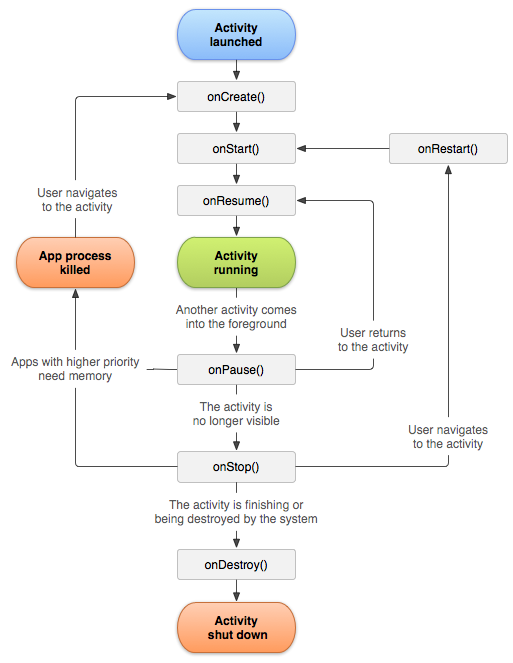
\includegraphics[scale=0.4]{04-framework/activity_lifecycle.png} 
   \caption{Ciclo de vida de una Activity}
   \label{fig:umlFrameworkCore}
\end{figure}


\subsection{Fragments}
Un Fragment representa una sección modular y reusable de la IU de una Activity, el cual se puede agregar o quitar mientras la Activity se esté ejecutando (algo así como una "sub-Activity"). Se pueden combinar varios Fragments en una sola Activity para crear una IU multipanel y volver a usar un Fragment en diferentes Activities.

Un Fragment define y administra su propio diseño, su propio ciclo de vida, y recibe sus propios eventos de entrada. Un Fragment no puede "vivir" por si mismo, debe ser hospedado por una Activity, y el ciclo de vida del Fragment se ve afectado directamente por el ciclo de vida de la Activity anfitriona. Por ejemplo, cuando la Activity está pausada, también lo están todos sus Fragments, y cuando la Activity se destruye, lo mismo ocurre con todos los Fragments.
\cite{androidDocs}

\begin{figure}[H]
  \centering
    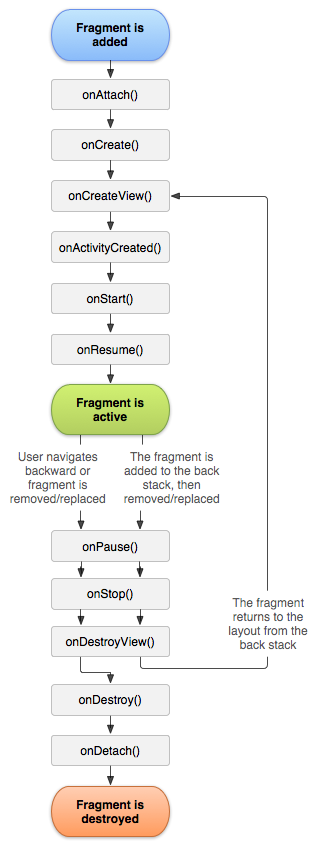
\includegraphics[scale=0.4]{04-framework/fragment_lifecycle.png} 
   \caption{Ciclo de vida de un Fragment}
   \label{fig:umlFrameworkCore}
\end{figure}

\subsection{Services}
...


\section{Estado del Arte}
\subsection{Sensr: un framework flexible para crear herramientas de recolección de datos con dispositivos móviles para ciencia ciudadana}

	Los dispositivos móviles son ideales para que las personas puedan de manera espontánea recolectar información. Sin embargo, esa simplicidad yace sobre una base que requiere fuertes conocimientos técnicos una infraestructura compleja. Por lo tanto, construir aplicaciones móviles implican una inversión que puede ser limitante para organizaciones pequeñas. Sensr es una herramienta que permite que personas que no son desarrolladoras tengan la posibilidad de crear herramientas que permitan la recolección de información para proyectos de ciencia ciudadana con dispositivos móviles. Esta herramienta aprovecha que el proceso y la estructura de la información en las actividades de recolección de datos de los proyectos de ciencia ciudadana son similares independientemente del dominio o la diversidad de los mismos. Sensr combina un ambiente de programación gráfico con una aplicación móvil para que las personas que no necesariamente poseen conocimientos técnicos puedan construir herramientas de recolección de información para dispositivos móviles y administrar la información recabada de manera colectiva.
	
	De esta manera, una persona que necesitan reunir información puede ser el autor de una campaña de ciencia ciudadana en el sitio de Sensr. La campaña es desplegada en la aplicación móvil de Sensr, y sus usuarios se pueden suscribir y contribuir a la campaña con los datos recolectados. Esta herramienta pretende simplificar de manera radical el proceso de crear una herramienta para dispositivos móviles que permita recolectar información y que sea de utilidad en una amplio conjunto de dominios de ciencia ciudadana. Los autores sólo necesitarían completar la descripción del proyecto y diseñar las plantillas o formularios que permitan el ingreso de los datos antes de incluir su proyecto en Sensr y ser distribuido de forma masiva. De esta manera, los autores se liberarían de las preocupaciones acerca de los requerimientos técnicos y las restricciones de la infraestructura.
	
	La falta de expertos técnicos y de recursos son a menudo los mayores obstáculos a la hora de desarrollar una aplicación móvil. Los grupos que quieren desarrollar una aplicación móvil de ciencia ciudadana a menudo son organizaciones sin fines de lucro o pequeñas organizaciones regionales que no poseen ni los recursos económicos ni los expertos técnicos que necesitan para desarrollar o mantener ese tipo de aplicaciones. Y además de la programación en si, la administración de los datos recolectados también representan un desafío, ya que estas mismas organizaciones tampoco poseen los servidores para almacenar o analizar el volumen de datos que puedan ser recolectados. El monitoreo participativo es un paradigma computacional que permite la recolección por parte de los voluntarios de información que se encuentra diseminada. Permite que el creciente número de usuarios de teléfonos móviles puedan compartir la información adquirida mediante los sensores de sus dispositivos en variados dominios. 
	
	Los investigadores han explorado la utilización de plataformas existentes como una alternativa para Y aunque varias de ellas son robustas y flexibles, la mayoría necesita de habilidad para programar y/o conocimiento de infraestructura en mayor o menor medida. Aunque por ejemplo el Proyecto Noah y EpiCollect son dos ejemplos claros de plataformas que soportan autoría de aplicaciones sin necesidad de programación. \cite{kim2013sensr}